% Options for packages loaded elsewhere
\PassOptionsToPackage{unicode}{hyperref}
\PassOptionsToPackage{hyphens}{url}
%
\documentclass[
  10pt,
  letterpaper,
  DIV=11,
  numbers=noendperiod,
  twoside]{scrartcl}

\usepackage{amsmath,amssymb}
\usepackage{setspace}
\usepackage{iftex}
\ifPDFTeX
  \usepackage[T1]{fontenc}
  \usepackage[utf8]{inputenc}
  \usepackage{textcomp} % provide euro and other symbols
\else % if luatex or xetex
  \usepackage{unicode-math}
  \defaultfontfeatures{Scale=MatchLowercase}
  \defaultfontfeatures[\rmfamily]{Ligatures=TeX,Scale=1}
\fi
\usepackage{lmodern}
\ifPDFTeX\else  
    % xetex/luatex font selection
  \setmainfont[ItalicFont=EB Garamond Italic,BoldFont=EB Garamond
Bold]{EB Garamond Math}
  \setsansfont[]{Europa-Bold}
  \setmathfont[]{Garamond-Math}
\fi
% Use upquote if available, for straight quotes in verbatim environments
\IfFileExists{upquote.sty}{\usepackage{upquote}}{}
\IfFileExists{microtype.sty}{% use microtype if available
  \usepackage[]{microtype}
  \UseMicrotypeSet[protrusion]{basicmath} % disable protrusion for tt fonts
}{}
\usepackage{xcolor}
\usepackage[left=1in, right=1in, top=0.8in, bottom=0.8in,
paperheight=9.5in, paperwidth=6.5in, includemp=TRUE, marginparwidth=0in,
marginparsep=0in]{geometry}
\setlength{\emergencystretch}{3em} % prevent overfull lines
\setcounter{secnumdepth}{3}
% Make \paragraph and \subparagraph free-standing
\ifx\paragraph\undefined\else
  \let\oldparagraph\paragraph
  \renewcommand{\paragraph}[1]{\oldparagraph{#1}\mbox{}}
\fi
\ifx\subparagraph\undefined\else
  \let\oldsubparagraph\subparagraph
  \renewcommand{\subparagraph}[1]{\oldsubparagraph{#1}\mbox{}}
\fi


\providecommand{\tightlist}{%
  \setlength{\itemsep}{0pt}\setlength{\parskip}{0pt}}\usepackage{longtable,booktabs,array}
\usepackage{calc} % for calculating minipage widths
% Correct order of tables after \paragraph or \subparagraph
\usepackage{etoolbox}
\makeatletter
\patchcmd\longtable{\par}{\if@noskipsec\mbox{}\fi\par}{}{}
\makeatother
% Allow footnotes in longtable head/foot
\IfFileExists{footnotehyper.sty}{\usepackage{footnotehyper}}{\usepackage{footnote}}
\makesavenoteenv{longtable}
\usepackage{graphicx}
\makeatletter
\def\maxwidth{\ifdim\Gin@nat@width>\linewidth\linewidth\else\Gin@nat@width\fi}
\def\maxheight{\ifdim\Gin@nat@height>\textheight\textheight\else\Gin@nat@height\fi}
\makeatother
% Scale images if necessary, so that they will not overflow the page
% margins by default, and it is still possible to overwrite the defaults
% using explicit options in \includegraphics[width, height, ...]{}
\setkeys{Gin}{width=\maxwidth,height=\maxheight,keepaspectratio}
% Set default figure placement to htbp
\makeatletter
\def\fps@figure{htbp}
\makeatother
% definitions for citeproc citations
\NewDocumentCommand\citeproctext{}{}
\NewDocumentCommand\citeproc{mm}{%
  \begingroup\def\citeproctext{#2}\cite{#1}\endgroup}
\makeatletter
 % allow citations to break across lines
 \let\@cite@ofmt\@firstofone
 % avoid brackets around text for \cite:
 \def\@biblabel#1{}
 \def\@cite#1#2{{#1\if@tempswa , #2\fi}}
\makeatother
\newlength{\cslhangindent}
\setlength{\cslhangindent}{1.5em}
\newlength{\csllabelwidth}
\setlength{\csllabelwidth}{3em}
\newenvironment{CSLReferences}[2] % #1 hanging-indent, #2 entry-spacing
 {\begin{list}{}{%
  \setlength{\itemindent}{0pt}
  \setlength{\leftmargin}{0pt}
  \setlength{\parsep}{0pt}
  % turn on hanging indent if param 1 is 1
  \ifodd #1
   \setlength{\leftmargin}{\cslhangindent}
   \setlength{\itemindent}{-1\cslhangindent}
  \fi
  % set entry spacing
  \setlength{\itemsep}{#2\baselineskip}}}
 {\end{list}}
\usepackage{calc}
\newcommand{\CSLBlock}[1]{\hfill\break\parbox[t]{\linewidth}{\strut\ignorespaces#1\strut}}
\newcommand{\CSLLeftMargin}[1]{\parbox[t]{\csllabelwidth}{\strut#1\strut}}
\newcommand{\CSLRightInline}[1]{\parbox[t]{\linewidth - \csllabelwidth}{\strut#1\strut}}
\newcommand{\CSLIndent}[1]{\hspace{\cslhangindent}#1}

\setlength\heavyrulewidth{0ex}
\setlength\lightrulewidth{0ex}
\usepackage[automark]{scrlayer-scrpage}
\clearpairofpagestyles
\cehead{
  Brian Weatherson
  }
\cohead{
  Four Problems in Decision Theory
  }
\ohead{\bfseries \pagemark}
\cfoot{}
\makeatletter
\newcommand*\NoIndentAfterEnv[1]{%
  \AfterEndEnvironment{#1}{\par\@afterindentfalse\@afterheading}}
\makeatother
\NoIndentAfterEnv{itemize}
\NoIndentAfterEnv{enumerate}
\NoIndentAfterEnv{description}
\NoIndentAfterEnv{quote}
\NoIndentAfterEnv{equation}
\NoIndentAfterEnv{longtable}
\NoIndentAfterEnv{abstract}
\renewenvironment{abstract}
 {\vspace{-1.25cm}
 \quotation\small\noindent\rule{\linewidth}{.5pt}\par\smallskip
 \noindent }
 {\par\noindent\rule{\linewidth}{.5pt}\endquotation}
\KOMAoption{captions}{tableheading}
\makeatletter
\@ifpackageloaded{caption}{}{\usepackage{caption}}
\AtBeginDocument{%
\ifdefined\contentsname
  \renewcommand*\contentsname{Table of contents}
\else
  \newcommand\contentsname{Table of contents}
\fi
\ifdefined\listfigurename
  \renewcommand*\listfigurename{List of Figures}
\else
  \newcommand\listfigurename{List of Figures}
\fi
\ifdefined\listtablename
  \renewcommand*\listtablename{List of Tables}
\else
  \newcommand\listtablename{List of Tables}
\fi
\ifdefined\figurename
  \renewcommand*\figurename{Figure}
\else
  \newcommand\figurename{Figure}
\fi
\ifdefined\tablename
  \renewcommand*\tablename{Table}
\else
  \newcommand\tablename{Table}
\fi
}
\@ifpackageloaded{float}{}{\usepackage{float}}
\floatstyle{ruled}
\@ifundefined{c@chapter}{\newfloat{codelisting}{h}{lop}}{\newfloat{codelisting}{h}{lop}[chapter]}
\floatname{codelisting}{Listing}
\newcommand*\listoflistings{\listof{codelisting}{List of Listings}}
\makeatother
\makeatletter
\makeatother
\makeatletter
\@ifpackageloaded{caption}{}{\usepackage{caption}}
\@ifpackageloaded{subcaption}{}{\usepackage{subcaption}}
\makeatother
\ifLuaTeX
  \usepackage{selnolig}  % disable illegal ligatures
\fi
\usepackage{bookmark}

\IfFileExists{xurl.sty}{\usepackage{xurl}}{} % add URL line breaks if available
\urlstyle{same} % disable monospaced font for URLs
\hypersetup{
  pdftitle={Four Problems in Decision Theory},
  pdfauthor={Brian Weatherson},
  hidelinks,
  pdfcreator={LaTeX via pandoc}}

\title{Four Problems in Decision Theory}
\author{Brian Weatherson}
\date{2024}

\begin{document}
\maketitle
\begin{abstract}
In recent years the literature on decision theory has become disjointed.
There isn't as much discussion as there should be on how different
problems impact one another. This paper aims to bring together work on
problems involving demons, problems about attitudes to risk, problems
about incomplete preferences, and problems about dynamic choice. In the
first three of these cases, I end up defending a pre-existing view. I
defend a ratificationist approach to problems with demons, the orthodox
expected utility approach to risk, and the permissibility of incomplete
preferences. These views are familiar, but seeing how they are related
to a common strengthens the case for each of them. The most novel part
of the view is the theory of dynamic choice that I offer: a sequence of
choices is rational only if both the so-called `resolute' and
`sophisticated' theories of dynamic choice would permit it. This theory
would be implausible if paired with many rival solutions to the first
three problems, but fits nicely with the view I'll develop through the
paper.
\end{abstract}

\setstretch{1.1}
Contemporary decision theory has become disjointed. There is less
overlap than there should be in work on adjacent problems. This paper
aims to undo some of that, by showing that four problems that have
largely been worked on in isolation cast useful light on each other. In
particular, I'll argue that we can go a long way towards solving all
four problems by working through the consequences of a plausible
principle that I'll call the Single Choice Principle.

The Single Choice Principle (hereafter, SCP) relates theories of static
choice and dynamic choice. In particular, it says that for a narrow
class of games, it doesn't matter whether you think of the game as
involving a static, strategic choice, or a dynamic choice that is made
during a game. One way into the principle is to think about an oddity in
the way Newcomb's Problem is normally introduced.

\section{Newcomb's Problem}\label{sec-newcomb}

\subsection{Standard Version}\label{sec-newcomb-standard}

In the standard vignette that goes with Newcomb's Problem, it is a
dynamic game. The demon makes a \emph{prediction}, and then the human
(hereafter, Chooser) makes a choice. Chooser doesn't know what Demon
did, but they do know that Demon has acted. So the natural presentation
of Newcomb's Problem is in a tree like
Figure~\ref{fig-standard-newcomb}.\footnote{I'll assume \$1,000 is worth
  1 util. I think this assumption of constant marginal utility is close
  to incoherent, and it will get relaxed later, but it's harmless for
  now.}

\subsection{Tree}

\begin{figure}

\centering{

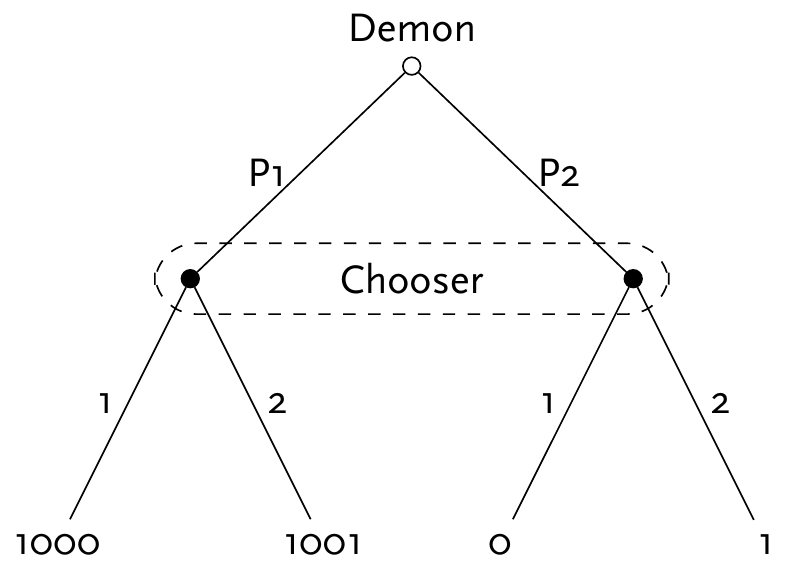
\includegraphics{fourprob_files/figure-pdf/fig-standard-newcomb-1.png}

}

\caption{\label{fig-standard-newcomb}Newcomb's Problem.}

\end{figure}%

\subsection{Table}

\begin{longtable}[]{@{}ccc@{}}
\caption{Newcomb's Problem}\label{tbl-standard-newcomb}\tabularnewline
\toprule\noalign{}
& P1 & P2 \\
\midrule\noalign{}
\endfirsthead
\toprule\noalign{}
& P1 & P2 \\
\midrule\noalign{}
\endhead
\bottomrule\noalign{}
\endlastfoot
1 & 1000 & 0 \\
2 & 1001 & 1 \\
\end{longtable}

I'll go over the details of how to read diagrams like
Figure~\ref{fig-standard-newcomb} in \textbf{?@sec-dualmandate}. All you
need to know for now is that the game starts at the open node, here at
the top, and it moves along by the agent (Demon or Chooser) making
choices. The dotted lines around the two nodes where Chooser acts mean
that those two nodes are in the same \textbf{information set}. That is,
when Chooser is at either one of those nodes, the strongest thing
Chooser knows is that they are somewhere or other in the set.\footnote{This
  formalism only really makes sense if we presuppose the right epistemic
  logic is S5, and there are good reasons to not make that assumption in
  general (\citeproc{ref-Humberstone2016}{Humberstone 2016, 380--402}).
  For this paper we'll treat it as a simplifying assumption that really
  should be relaxed in subsequent work.} So this tree represents the
standard vignette for Newcomb's Problem. Demon makes a prediction - I'm
in general using PX for Demon predicting X - and Chooser knows that the
prediction has been made, and that either P1 or P2 happened, but chooses
without knowing which it is. Then the game is resolved.

What Table~\ref{tbl-standard-newcomb} shows is a subtly different story.
In Table~\ref{tbl-standard-newcomb}, each player chooses a
\emph{strategy}. A strategy for a player in a tree like
Figure~\ref{fig-standard-newcomb} is a decision about what to do at each
node in the tree where that player has to move.\footnote{In game theory,
  it is usually specified that strategies include decisions about what
  to do at nodes that are ruled out by earlier moves in that very
  strategy. In theory I'm assuming this whenever I talk about
  strategies; in practice it doesn't matter for any application in this
  paper.} So what Table~\ref{tbl-standard-newcomb} represents is a
situation where each player chooses a strategy simultaneously, and that
determines a result for the game. It differs from
Figure~\ref{fig-standard-newcomb} in part in that it's symmetric; there
is no hint that Demon moves first.

There is a lot of disagreement about Newcomb's Problem, but here is one
point of universal agreement: Figure~\ref{fig-standard-newcomb} and
Table~\ref{tbl-standard-newcomb} have the same solutions. It would be
incoherent to prefer taking 1 box in one of these puzzles and 2 boxes in
the other, or to say that both options were choice-worthy in one puzzle
but not the other. They may not represent exactly the same problem, they
don't pose exactly the same question to Chooser, but they should get the
same answer (or answers).

I'm going to agree with the unanimous verdict on this point, but I'll
start dissenting from orthodox opinion very soon. And one way into my
dissent is to ask, why should Figure~\ref{fig-standard-newcomb} and
Table~\ref{tbl-standard-newcomb} get the same answer? What principle is
someone who gives different answers to the two questions violating? I
have a suggestion for what principle that might be, the SCP, but to make
that suggestion plausible we need a couple more examples.

\subsection{Variant 1: Coin-then-Demon}\label{variant-1-coin-then-demon}

Consider a variant on Newcomb's Problem I'll call Coin-Then-Demon. In
this game a fair coin will be flipped and shown to Demon and Chooser. If
it lands Heads, Chooser will get \$5,000 and the game ends. Otherwise,
they play standard Newcomb Problem. Figure~\ref{fig-coin-then-demon}
shows the game tree for this game, with Nature moving first, and the
probabilities of Nature's moves shown. And
Table~\ref{tbl-coin-then-demon} shows the strategy table for it, with
the payouts shown in expected value.\footnote{I will drop the assumption
  that Chooser maximises expected value in \textbf{?@sec-buchak}, but
  it's a harmless assumption for now.}

\subsection{Tree}

\begin{figure}

\centering{

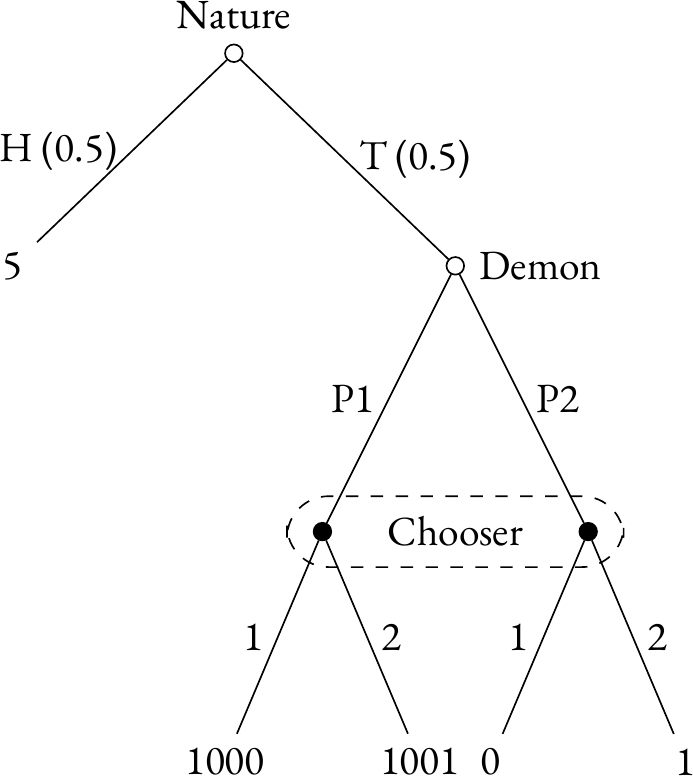
\includegraphics{fourprob_files/figure-pdf/fig-coin-then-demon-1.png}

}

\caption{\label{fig-coin-then-demon}Coin-then-Demon}

\end{figure}%

\subsection{Table}

\begin{longtable}[]{@{}ccc@{}}
\caption{Coin-then-Demon}\label{tbl-coin-then-demon}\tabularnewline
\toprule\noalign{}
& P1 & P2 \\
\midrule\noalign{}
\endfirsthead
\toprule\noalign{}
& P1 & P2 \\
\midrule\noalign{}
\endhead
\bottomrule\noalign{}
\endlastfoot
1 & 502.5 & 2.5 \\
2 & 503 & 3 \\
\end{longtable}

I have two hypotheses about
Figure~\ref{fig-coin-then-demon}/Table~\ref{tbl-coin-then-demon}; one of
which I think everyone will agree with, and one that might be more
controversial. The less controversial hypothesis is that in this game,
as in standard Newcomb's Problem, it doesn't matter whether Chooser is
playing the dynamic game (i.e., Figure~\ref{fig-coin-then-demon}) or the
strategic game (i.e., Table~\ref{tbl-coin-then-demon}). Whichever
options are choice-worthy in one are choice-worthy in the other. The
more controversial hypothesis is that the reason these two games are
rationally equivalent is exactly the same as the reason that the two
forms of Newcomb Problem I presented should get the same answer.

\subsection{Variant 2: Demon-then-Coin}\label{variant-2-demon-then-coin}

One more example and we're basically done. In the game I'll call
Demon-Then-Coin, the coin is only flipped if Demon predicts Chooser
takes one box. If the coin lands heads, Chooser gets \$5,000, and the
game ends. If either Demon predicts 2 boxes, or the coin lands tails,
Chooser makes a selection, knowing that one or other of these disjuncts
obtained. Then the game ends. The tree for this game is
Figure~\ref{fig-demon-then-coin}, and the strategy table is
Table~\ref{tbl-demon-then-coin}.

\subsection{Tree}

\begin{figure}

\centering{

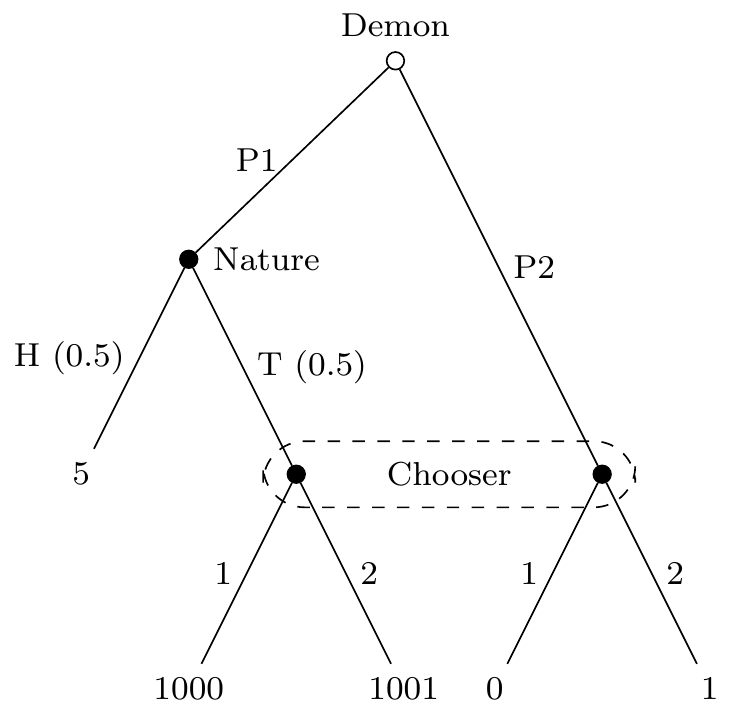
\includegraphics{fourprob_files/figure-pdf/fig-demon-then-coin-1.png}

}

\caption{\label{fig-demon-then-coin}Demon-then-Coin}

\end{figure}%

\subsection{Table}

\begin{longtable}[]{@{}ccc@{}}
\caption{Demon-then-Coin}\label{tbl-demon-then-coin}\tabularnewline
\toprule\noalign{}
& P1 & P2 \\
\midrule\noalign{}
\endfirsthead
\toprule\noalign{}
& P1 & P2 \\
\midrule\noalign{}
\endhead
\bottomrule\noalign{}
\endlastfoot
1 & 502.5 & 0 \\
2 & 503 & 1 \\
\end{longtable}

If Chooser was planning on picking 1 box, they have a little evidence
against the accuracy of Demon's predictions. If in the other games they
thought the probability that Demon mispredicted was \emph{e}, in this
case they should (if they plan to choose 1 box) have a probability of
error of roughly 2\emph{e}. But if \emph{e} was small enough to start
with, and I'll assume throughout that Demon's error likelihood is
arbitrarily small, this shouldn't make a difference.

Again, I'm going to argue that the dynamic game,
Figure~\ref{fig-demon-then-coin}, and the strategic game,
Table~\ref{tbl-demon-then-coin}, should get the same solutions. Indeed,
they should get the same solutions for the same reason the previous two
pairs of decisions should get the same solutions. That reason, I'll
argue, is the Single Choice Principle.

\subsection{Single Choice Principle}\label{sec-scp-definition}

Here is what the Single Choice Principle (hereafter, SCP) says:

\begin{quote}
\textbf{Single Choice Principle (SCP)}\\
In any decision tree in which all the nodes where Chooser acts are in a
single information set, an option is choice-worthy in the dynamic form
of the game iff it is choice-worthy in the strategic form of the game.
\end{quote}

The SCP is a highly restricted version of a claim that dynamic and
static games are in some sense equivalent. The strong version of the
view says that there is some mapping from the set of rational choices in
a tree to the set of possible choices in the strategic version of that
tree. Exactly how that mapping should be understood is tricky in the
general case, but since (a) the general principle is extremely
controversial, and (b) I'm not endorsing the general principle, I won't
fuss over the details. What I will fuss over is getting clearer about
what the SCP does and doesn't say.

The SCP doesn't just say that on any run through the game, Chooser only
makes one choice. Rather, it says that Chooser only has one possible
choice to make in the game. This point might be clearer with an example.
Imagine Chooser and Demon are playing a simple kind of ultimatum game.
Demon has to propose a split of a \$3 pot; they can either propose \$2
for Demon and \$1 for Chooser, or vice versa. Chooser then has a take it
or leave it choice. If they take, each party gets the money Demon
proposes; if they leave, each party gets \$0. Assume Demon is
arbitrarily good at predicting Chooser's strategy, and that Demon
prefers more money to less\footnote{Also assume Demon will flip a coin
  if they expect each option to have equal return}. The game tree is in
Figure~\ref{fig-ultimatum}, and the strategy table is in
Table~\ref{tbl-ultimatum}.

\subsection{Tree}

\begin{figure}

\centering{

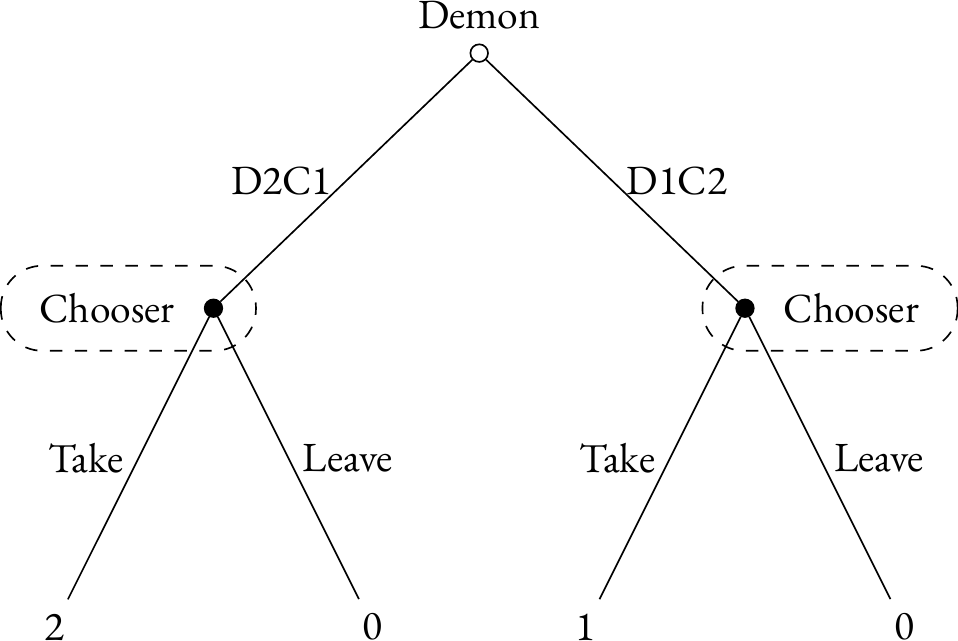
\includegraphics{fourprob_files/figure-pdf/fig-ultimatum-1.png}

}

\caption{\label{fig-ultimatum}Ultimatum Game}

\end{figure}%

\subsection{Table}

\begin{table}

\caption{\label{tbl-ultimatum}Two representations of the strategic form
of ultimatum game}

\begin{minipage}{0.50\linewidth}

\subcaption{\label{tbl-ultimatum-game}Demon's Decisions}

\centering{

\begin{tabular}{ccc}
\toprule
 & D2C1 & D1C2\\
\midrule
\textbf{TT} & 1 & 2\\
\textbf{TL} & 1 & 0\\
\textbf{LT} & 0 & 2\\
\textbf{LL} & 0 & 0\\
\bottomrule
\end{tabular}

}

\end{minipage}%
%
\begin{minipage}{0.50\linewidth}

\subcaption{\label{tbl-ultimatum-demon}Demon's Predictions}

\centering{

\begin{tabular}{ccccc}
\toprule
 & PTT & PTL & PLT & PLL\\
\midrule
\textbf{TT} & 1 & 1 & 2 & 1.5\\
\textbf{TL} & 1 & 1 & 0 & 0.5\\
\textbf{LT} & 0 & 0 & 2 & 1\\
\textbf{LL} & 0 & 0 & 0 & 0\\
\bottomrule
\end{tabular}

}

\end{minipage}%

\end{table}%

Most philosophers would say that in the dynamic form of the game,
Figure~\ref{fig-ultimatum}, the only sensible thing to do is TT;
whatever the demon does, it's better to take more money than less. But
many would also say that in the strategic form,
Table~\ref{tbl-ultimatum}, some other strategy might be appropriate. For
instance, Evidential Decision Theory says that in
Table~\ref{tbl-ultimatum}, the right strategy is LT.\footnote{This is
  easier to see in Table~\ref{tbl-ultimatum-demon}; EDT says to just
  look at the numbers in the main diagonal and choose the strategy with
  the highest one.} The SCP does not rule out this combination. It will
ultimately have something to say about EDT, but it doesn't object to
this pair of views. That's because in Figure~\ref{fig-ultimatum} there
are two possible choices for Chooser to make, even if they will
ultimately only make one of them, and the SCP only applies to games with
just one possible choice. That makes it a more plausible principle, but
surprisingly does little to reduce its philosophical significance.

\section{Defending the SCP}\label{sec-scp-defence}

\subsection{A Sample Violation}\label{a-sample-violation}

The argument for the SCP is that violations of it are in various ways
incoherent. It helps to have a sample violation on the table. Imagine
Chooser is going to play the following game.

\begin{figure}

\centering{

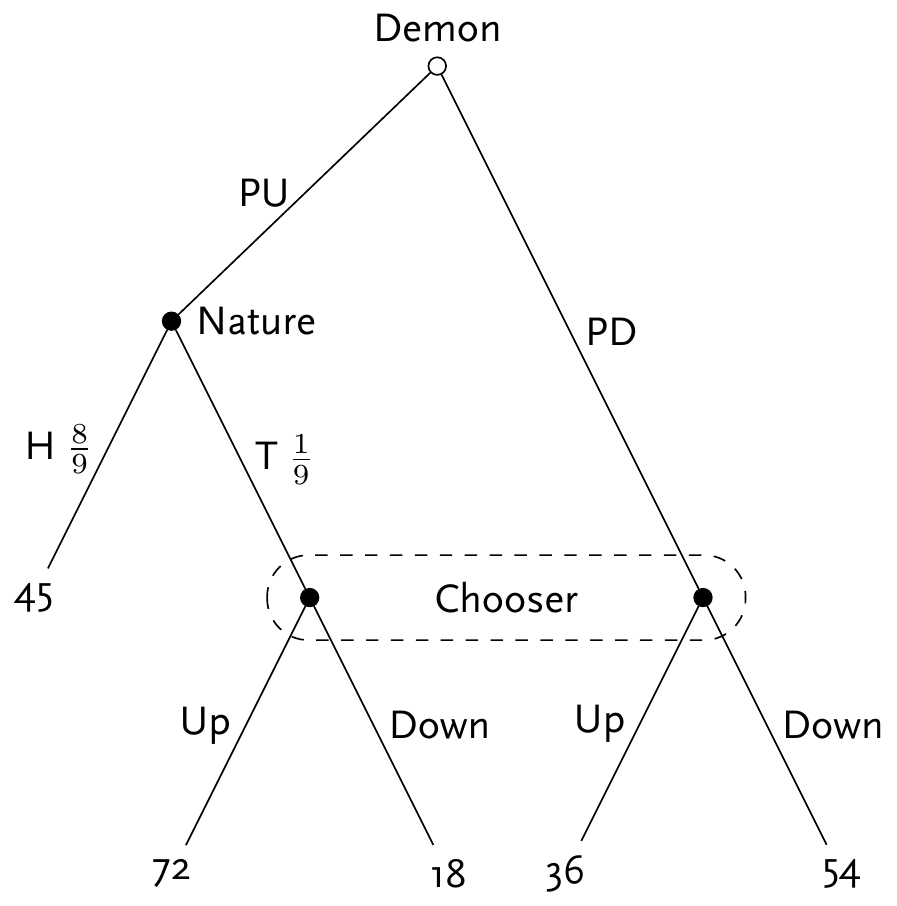
\includegraphics{fourprob_files/figure-pdf/fig-sample-violation-1.png}

}

\caption{\label{fig-sample-violation}Switching Example}

\end{figure}%

Figure~\ref{fig-sample-violation} resembles
Figure~\ref{fig-demon-then-coin}, with two notable differences. First,
the coin is now weighted, and has an 8/9 chance of landing Heads.
Second, if Chooser must choose, either option is an equilibrium.

Table~\ref{tbl-sample-violation-late} shows the decision table Chooser
faces if they must make a choice in Figure~\ref{fig-sample-violation},
and \textbf{?@tbl-sample-violation-early} shows the expected payouts of
the two strategies Chooser could select.

\begin{table}

\caption{\label{tbl-sample-violation}Payout tables for
Figure~\ref{fig-sample-violation}.}

\begin{minipage}{0.50\linewidth}

\subcaption{\label{tbl-sample-violation-late}Dynamic version.}

\centering{

\begin{tabular}{ccc}
\toprule
 & PU & PD\\
\midrule
\textbf{Up} & 72 & 36\\
\textbf{Down} & 18 & 54\\
\bottomrule
\end{tabular}

}

\end{minipage}%
%
\begin{minipage}{0.50\linewidth}

\subcaption{\label{tbl-sample-violation-late}Strategic version.}

\centering{

\begin{tabular}{ccc}
\toprule
 & PU & PD\\
\midrule
\textbf{Up} & 48 & 36\\
\textbf{Down} & 42 & 54\\
\bottomrule
\end{tabular}

}

\end{minipage}%

\end{table}%

I'll take as my sample violator of the SCP a Chooser who prefers Up in
the dynamic version, and Down in the strategic version. As we'll see in
\textbf{?@sec-multiple}, many decision theorists agree with this
Chooser. But everything I say should generalise to any violation.

\subsection{Ramsey Test}\label{sec-ramsey}

To choose a strategy is to make true a bunch of conditionals. Adopting
the strategy Down in Figure~\ref{fig-sample-violation} just is saying
``If I have to choose, I'll choose Down''. As
(\citeproc{ref-RamseyTest}{\textbf{RamseyTest?}}) said, the way to tell
which such conditional to make true is to hypothetically add the
antecedent to one's stock of belief, and then decide which unconditional
claim you'd like to make true. But Chooser does not do that. If they
believed that they had to choose, they would choose Up. So their
strategic preference implies that they believe that if they had to
choose, they would choose Down, but adding the supposition that they
have to choose, they choose Up. This combination is incoherent, and so
violations of the SCP are incoherent.

I think this argument is decisive; it's incoherent to adopt a strategy
in games like Figure~\ref{fig-demon-then-coin} or
\textbf{?@fig-switching-example} that is different from what one knows
one would do if one had to carry the strategy out. That's just not how
conditionals work. But in case not everyone is convinced, I'll run
through some other arguments. The SCP will do a lot of work, and it is
worth getting the foundations as secure as possible.

\subsection{Intuitions about Change}\label{intuitions-about-change}

This argument starts with a story. Imagine the game master (GM) is
chatting to Chooser (C), before Chooser plays
\textbf{?@fig-switching-example}.

\begin{quote}
GM: What are you thinking of playing?\\
C: I might not have a choice.\\
GM: True, but assume you have to choose.\\
C: Then Up, I guess.\\
GM: You know, Demon can be really slow in making a prediction. Do you
want to write your choice down in an envelope, and we'll open it if it's
needed? C: Oh sure. I'm writing Down.\\
GM: Why did you change your mind?
\end{quote}

We could continue the conversation, but I want to focus on the
presupposition of GM's last question. It seems appropriate to presuppose
here that Chooser has changed their mind. This presupposition requires
the SCP. If the SCP is false, Chooser has simply given different answers
to different questions. First they were asked what to do in the dynamic
game, and they said Up. Then they were asked what to do in the strategic
game, and they said Down. Giving different answers to different
questions is not changing one's mind.

GM's question seems appropriate. Chooser was first asked what they
planned to do in a particular situation. Then they were asked for a
strategy that would only be activated in that very situation. When they
give different answers to those questions, it sounds like they changed
their mind. That implies the questions are fundamentally the same, which
is what the SCP says.

\subsection{Unifying the Examples}\label{sec-unity}

Philosophers do not agree about Newcomb's Problem. But they do agree
that in each of the examples in Section~\ref{sec-newcomb}, the same
choice is rational in the strategic and dynamic form of the game. This
isn't because they think that in general strategic and dynamic forms are
equivalent. Indeed, for many theorists there is no unifying story about
why each of these pairs of problems gets the same answer. It is just a
fact that the theory treats the dynamic and strategic problems the same
way.

I think it is better to have an explanation for why each of the pairs of
problems gets the same answers, and for that explanation to be the same
across the three pairs. The SCP provides such an explanation, and that's
a point in its favour.

\subsection{No Reward}\label{no-reward}

One reason that I introduced
Figure~\ref{fig-ultimatum}/Table~\ref{tbl-ultimatum} earlier is that
it's the kind of case where it's most plausible that the strategic and
dynamic choices might be distinct. Think about the pair of choices that
EDT recommends: in the dynamic game, play TT; in the strategic game,
play LT. While I ultimately disagree with this, I do think this is a
plausible thing for EDT to say. The strategy LT has two big advantages
that some will think make up for the fact that it is not what one would
do dynamically. First, it differs from the dynamically rational play
only in a situation which is, conditional on being played, highly
unlikely to come about. Second, there is a reward, at least in
expectation, for playing this dynamically irrational strategy; the
strategy has a payout of 2 while the dynamically rational strategy only
has a payout of 1. Either one of these facts will, at least to some
people, make it rational to treat dynamic and strategic games
differently; what's distinctive about
Figure~\ref{fig-ultimatum}/Table~\ref{tbl-ultimatum} is that both
reasons are there.

In dynamic problems where the SCP applies, neither of these reasons can
apply. There is no possible strategic advantage to playing the
dynamically irrational strategy. There is no parallel to saying, ``I'm
playing LT because, even though leaving money would be irrational, I
almost certainly won't have to carry that part of the strategy out, and
in exchange for this tiny risk, I'm getting rewarded.'' Doing something
dynamically irrational at the only point one can possibly move can't
have advantages elsewhere; you're going to get the same payout elsewhere
no matter what. So whatever reason one could have in other cases for
treating dynamic and strategic problems separately can't apply here;
there isn't enough of an `elsewhere' for one's bad decision at the one
and only place one moves to be compensated.

\subsection{Sure Thing}\label{sec-surething}

Finally, there is one very natural argument for the SCP that for various
reasons I don't want to lean on too heavily. If Chooser violates the
SCP, then they violate the Sure Thing Principle. They think Up is at
least as good as Down both conditional on the game ending without them
making a choice, and on that not happening. But they think Down is
better overall. If Sure Thing can be taken as a basic assumption, the
SCP immediately follows.

There are three problems with this line of reasoning. The first is
pragmatic. It's well known that various theories I'm arguing against
here, like EDT, and Buchak's non-standard treatment of risk, violate
Sure Thing. It's not a new argument against them to say that they
violate the SCP, if the only reason to believe the SCP is Sure Thing.
The second is that it isn't obvious that the theories that are best
supported by the SCP are not consistent with Sure Thing. Dmitri
(\citeproc{ref-Gallow202x}{\textbf{Gallow202x?}}) argues that what he
calls `stable' decision theories are bound to violate Sure Thing. It's
arguable that his arguments can be generalised to provide a reason to
think theories supported by the SCP (which will typically not be stable
in his sense) also violate Sure Thing. And the third is that even if
this argument fails, there is a bad company objection to Sure Thing that
I'll get to in \textbf{?@sec-negdom}. So it's useful that we have the
other four arguments to fall back on.

\phantomsection\label{refs}
\begin{CSLReferences}{1}{0}
\bibitem[\citeproctext]{ref-Humberstone2016}
Humberstone, Lloyd. 2016. \emph{Philsophical Applications of Modal
Logic}. Milton Keynes: College Publications.

\end{CSLReferences}



\noindent Unpublished. Posted online in 2024.

\end{document}
